\documentclass[9 pt]{beamer}
\usepackage[utf8]{inputenc}
\usepackage[T1]{fontenc}
\usepackage{bm}
\usepackage{array}
\usetheme{tullia}

\begin{document}



\begin{frame}

\begin{tikzpicture}[remember picture,overlay] % Background box
\node [xshift=\paperwidth/2,yshift=\paperheight/2] at (current page.south west)[rectangle,fill,inner sep=0pt,minimum width=\paperwidth,minimum height=3*\paperheight/5,top color=light,bottom color=light]{}; % Change the height of the box, its colors and position on the page here
\end{tikzpicture}



\color{white}\sffamily

\hfill \huge{Wasserstein Consensus \\ \hfill for Bayesian Sample Size Determination}
\vspace{0.6cm}


\begin{columns}

\begin{column}{0.45\textwidth}
\vspace{1.55cm}


\includegraphics[width=.7\textwidth]{sapienza-logo-png-6.png}

{\small Dipartimento di Scienze Statistiche}

\end{column}

\begin{column}{0.45\textwidth}

\hfill \Large{Tullia Padellini}

\vspace{0.25cm}


\hfill \scriptsize{tulliapadellini.github.io     \faLaptop} 

\hfill \scriptsize{tullia.padellini@uniroma1.it   \faEnvelope}

\vspace{0.5cm}
\vspace{0.3cm}

\small{\hfill \faUserPlus \; Michele Cianfriglia \\ \hfill Pierpaolo Brutti } 



\vspace{0.7cm}
\vfill
\hfill Napoli -- 9 July 2019 
\end{column}

\end{columns}


\end{frame}





\begin{frame}{Sample Size Determination}
\framesubtitle{the big picture}

Pre-sperimental problem consisting of \textbf{choosing the
size of the sample, $n$}, typically trying to minimize uncertainty under some cost constraint. 

\pause
\vspace{0.75cm}

In \textcolor{light}{\bf Clinical Trials} this translates into:

\begin{itemize}
\tightlist
\item \textbf{Cost} - every patient is "precious" for both ethics and finances
\item \textbf{Uncertainty} - we cannot risk introducing a dangerous treatment
\end{itemize}


\pause
\begin{exampleblock}

\textbf{GOAL:} find a sample size that induces agreement between different parties

\end{exampleblock}

\end{frame}


\begin{frame}{The (bayesian) state of the art}
\framesubtitle{the main ingredients}

%$\theta$ 

\begin{itemize}
    \item Analysis Prior $\pi_A(\theta)$:
    \begin{itemize}
        \item \textcolor{light}{models pre-experimental information to be used to obtain the\\ {\bf posterior distribution}}
    \end{itemize}
    \vspace{0.25cm}

    \item Design Prior $\pi_D(\theta)$:
    \begin{itemize}
        \item \textcolor{light}{models uncertainty on the experiment to be used to obtain the\\ {\bf predictive distribution}}
    \end{itemize}
\end{itemize}

\pause
\vspace{0.5cm}

\begin{exampleblock}

Select $n$ in order to satisfy some inferential goal, to be formalized in terms of a summary of the posteriors
\[\rho_{\pi_A}(\theta|y_n) = \int{ g(\theta)\pi_A(\theta|y_n)\text{d}\theta } \]

\end{exampleblock}

\end{frame}

\begin{frame}{The (bayesian) state of the art}
\framesubtitle{in the two prior approach}

The design predictive distribution $m_D(y)$ removes the dependency of $\rho_{\pi_A}(\theta|y_n)$ from the observed sample $y_n$

\vspace{0.35cm}

\begin{itemize}
    \item<2->  \textcolor<3->{gray}{ \textcolor<2>{light}{\bf PEC} - Predictive Expectation Criterion}
    \begin{itemize}
        \textcolor<3->{gray}{\item<2->  \[ e(n) = \mathbb{E}_{m_D}[ \rho_{\pi_A}(\theta|Y_n)]  \qquad \qquad n^* = \min \{n \in \mathbb{N} : e(n)> \eta\}\]}
    \end{itemize}

    \item<3->         \textcolor<4->{gray}{\textcolor<3>{light}{\bf PPC} - Predictive Probability Criterion}
    
        \begin{itemize}
                \textcolor<4->{gray}{\item<3->  \[         p(n) = \mathbb{P}_{m_D}[\rho_{\pi_A}(\theta|Y_{n}) > \gamma]  \qquad \qquad n^* = \min \{n \in \mathbb{N} : p(n)> \eta\}\]}
    \end{itemize}
\end{itemize}

\pause 
\pause
\pause
$\eta$ and $\gamma$ are clinically relevant thresholds and depend on the problem.
\end{frame}

\begin{frame}{Multiple priors}
\protect\hypertarget{multiple-priors}{}

\framesubtitle{when should we look for "consensus"? }

\begin{itemize}
\item diverging expert opinions
\item multiple scenarios to take into account
\item data from previous studies
\end{itemize}

\vspace{0.75cm}
\pause


\textbf{\color{light} Community of priors problem}: how to combine multiple sources of pre-sperimental information into the analysis? 

\end{frame}

\begin{frame}{The standard Solution}
\protect\hypertarget{the-standard-solution}{}

\framesubtitle{mixtures of priors}

Aggregate multiple priors into one and then use the approach of your likings. 

\vspace{0.5cm}

\pause


 \[\pi_1(\theta), \dots, \pi_K(\theta)\quad
    \uncover<3-> {
    \textcolor{gray}{\xrightarrow{\hspace*{1.5cm}}} \quad
    \pi_A (\theta) = \sum_{i=1} ^ K \omega_{0,i} \pi_i(\theta)
    }
\]

\pause

\pause

\[ \pi_A(\theta|y_n) = \sum_{i = 1} ^K {\frac{\omega_{0,i} m_i(y_n)}{\sum_{r = 1} ^K \omega_{0,r} m_r(y_n)} \times \pi_i(\theta|y_n)}  \]

\pause

\begin{exampleblock}

\begin{center}
Will the $i$-th clinician believe us? 
\end{center}
\end{exampleblock}

\textcolor[RGB]{220,220,220}{\rule{\linewidth}{0.2pt}}

\tiny{\faBook \;Brutti, P., De Santis, F., \& Gubbiotti, S. (2009). \textit{Mixtures of prior distributions for predictive Bayesian sample size calculations in clinical trials}. Statistics in medicine}

\end{frame}



\begin{frame}{Our Solution}
\framesubtitle{enforcing ``consensus'' between sources}

\begin{itemize}
    \item (possibly) conflicting priors $\pi_1 , \pi_2$
    \item resulting posteriors $\pi_{1,y}, \pi_{2,y}$
\end{itemize}

\vspace{0.5cm}
Two experts ``agree'' if their inferential conclusions are the same\uncover<2->{, hence if their \textbf{\color{light} posterior distributions are close enough}. 
}
\vspace{0.5cm}

\pause 
\pause

\begin{exampleblock}

\begin{center}
    
We formalize \textbf{\color{light} agreement} or \textbf{\color{light}consensus} in terms of\\ distance between $\pi_{1,y}$ and $\pi_{2,y}$
\end{center}
\end{exampleblock}




\end{frame}

\begin{frame}{Formally}{how does this relate to the standard framework?}

We can still adopt the Predictive approach, as this it's just another way of defining the summary statistic: $$\rho_{\pi_A}(\theta|y_n) \quad \uncover<2-> { \textcolor{gray}{\xrightarrow{\hspace*{1cm}}}\quad d(\pi_{1,y}, \pi_{2,y})
}$$


\vspace{0.3cm}

\begin{itemize}
    \item<3->  \textcolor<4->{gray}{ \textcolor<3>{light}{\bf PEC} - Predictive Expectation Criterion}
    \begin{itemize}
        \textcolor<4->{gray}{\item<2->  \[ e_{1,2}(n) = \mathbb{E}_{m_D}[ d(\pi_{1,y}, \pi_{2,y})]  \qquad \qquad n^* = \min \{n \in \mathbb{N} : e_{1,2}(n) \bm{<} \eta\}\]}
    \end{itemize}

      \item<4->         \textcolor<5->{gray}{\textcolor<4>{light}{\bf PPC} - Predictive Probability Criterion}
    
        \begin{itemize}
                \textcolor<5->{gray}{\item<4->  \[         p_{1,2}(n) = \mathbb{P}_{m_D}[d(\pi_{1,y}, \pi_{2,y}) > \gamma]  \qquad \qquad n^* = \min \{n \in \mathbb{N} : p_{1,2}(n) \bm{<} \eta\}\]}
    \end{itemize}
\end{itemize}

\pause
\pause
\pause
\pause

%
\begin{center}
\textbf{\color{light} we just need to pick a distance}
\end{center}

\end{frame}

\begin{frame}{Wasserstein distance}
\framesubtitle{a.k.a. Kantorovic, Earth Mover}
\begin{columns}

\begin{column}{0.49\textwidth}

\textbf{\color{light} $(p,d)-$ Wasserstein distance}
\vspace{0.25cm}

$X \sim {P}$ and $Y \sim {Q}$, $p \geqslant 1$ and $d$ ground distance $$W_{d, p}(P,Q) = \left( \inf_{J}  \int_{\mathcal{X} \times \mathcal{Y}} \!\!\!\!\!\! d(x,y)^{p} \,\,\, \text{d}J(x,y)\right)^{1/p}$$ where the infimum is over \textbf{all joint} distributions $\text{J}$ having $P$ and $Q$ as marginals.
\end{column}

\begin{column}{0.49\textwidth}
\begin{figure}
    \centering
    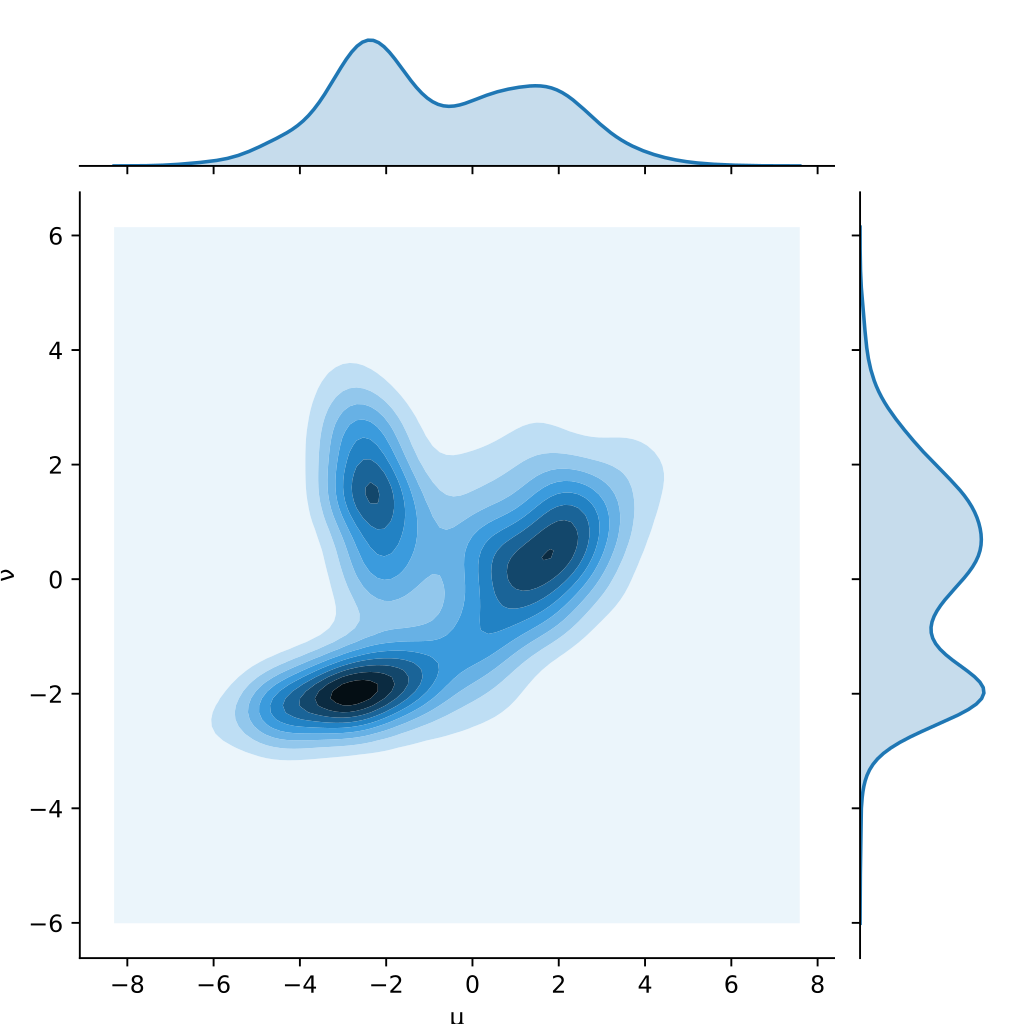
\includegraphics[width = .9\textwidth]{images/transp-plan.png}
\end{figure}

\end{column}

\end{columns}

%\vspace{0.5cm}
%Usually $L_p$ norm as ground metric


\end{frame}
\begin{frame}{Wasserstein distance}{it's this popular for a good reason}
\begin{itemize}
\tightlist
\item<1-> it ``metricises'' convergence in distribution
  \begin{itemize}
      \item<1-> \textcolor{light}{if two distributions are close w.r.t. the Wasserstein distance they are probabilistically similar.} 
  \end{itemize}
\vspace{0.5cm}


\item<2-> it tells us why the distributions differ
\begin{itemize}
    \item<2-> \textcolor{light}{with the Wasserstein distance is associated to a map (transport plan) that shows us how we have to move the mass of P to morph it into Q.}
\end{itemize}
\vspace{0.5cm}


\item<3->
  it is sensible to the geometry of the space
  \begin{itemize}
      \item<3-> \textcolor{light}{it's not just about the location!}
  \end{itemize}

\end{itemize}

\vspace{0.75cm}
\textcolor[RGB]{220,220,220}{\rule{\linewidth}{0.2pt}}
\tiny{\faBook \; Verdinelli, I., Wasserman, L. (2018) Hybrid Wasserstein Distance and Fast Distribution Clustering. \textit{arXiv preprint arXiv:1812.11026}}

\end{frame}

\begin{frame}{Multivariate Gaussian distributions}
\framesubtitle{computing the Wasserstein distance}
Let $X \sim \text{N}(\boldsymbol{\mu}_{X}, \boldsymbol{\Sigma}_{X})$ and $Y \sim \text{N}(\boldsymbol{\mu}_{Y}, \boldsymbol{\Sigma}_{Y})$, when \textcolor{light}{\bf the ground distance is taken to be the $L_2$ distance}, we have a closed form expression for Wasserstein:
\vspace{0.25cm}

\[\text{W}_{L^2,2}(X,Y)  = \| \boldsymbol{\mu}_{X} - \boldsymbol{\mu}_{Y} \|_{2}^{2} + \mathtt{B}^{2}(\boldsymbol{\Sigma}_{X}, \boldsymbol{\Sigma}_{Y}) \]

\vspace{0.7cm}

\pause 
$\mathtt{B}^{2}(\boldsymbol{\Sigma}_{X}, \boldsymbol{\Sigma}_{Y}) = \text{tr}\left[\boldsymbol{\Sigma}_{X} + \boldsymbol{\Sigma}_{Y} - 2\sqrt{\boldsymbol{\Sigma}_{X}^{1/2}\boldsymbol{\Sigma}_{Y}\boldsymbol{\Sigma}_{X}^{1/2}}\,\right]$ is the \textbf{ \color{light} Bures distance}.

\vspace{.8cm}

 \pause

\begin{exampleblock}

\begin{center}
    distance between the means \textbf{+} distance between the variances
\end{center}

\end{exampleblock}
%\pause
%\vspace{0.15cm}
%It's interpretable \& fast to compute!
 
 \end{frame}
 
 \begin{frame}{Conjugate Univariate Gaussian Model}
\framesubtitle{computing the Wasserstein distance}

\textbf{Likelihood:} $\text{N}(\theta, \sigma^2)$, with $\sigma^2$ known.


\[ \textcolor<2->{black}{
\pi(\theta) =  \text{N}\left(\theta; \mu_0, \frac{\sigma^2}{n_0}\right)} 
\uncover<2-> {
\qquad \qquad \qquad 
\pi(\theta |y_n) = \text{N}\left(\theta; \frac{n_{0}\mu_{0} + n\overline{y}_{n}}{n + n_{0}}, \frac{\sigma^{2}}{n + n_{0}}\right)}\]

\pause
\pause

\vspace{0.5cm}
If we have two priors, Wasserstein between the corresponding posteriors is:

\vspace{0.35cm}


\begin{exampleblock}

\[
\text{W}_{L^2, 2}(\pi_{1,y} , \pi_{2,y})  = \left(\mu_{1,\mathtt{P}} - \mu_{2,\mathtt{P}}\right)^{2} + \left(\sigma_{1,\mathtt{P}} - \sigma_{2,\mathtt{P}}\right)^{2}.
\]
\end{exampleblock}

\end{frame}

\begin{frame}{Conjugate Gaussian Model}{in the Bayesian predictive approach to SSD}

Under the usual $\pi_D(\theta)\sim \text{N}(\mu_D, \sigma/n_D)$ assumption: 

\vspace{0.25cm}

\pause
 \[\text{\bf \color{light} PEC:}\qquad  e_{1,2}(n) = \widetilde{\mu}^{2} + \sigma^{2}\left(w_{n}^{2}\left[\frac{1}{n} + \frac{1}{n_{D}}\right] + \left[\frac{1}{\sqrt{n + n_{1}}} - \frac{1}{\sqrt{n + n_{2}}}\right]^{2}\right)\]

\pause
\vspace{0.5cm}

        \[\text{\bf \color{light} PPC:}\qquad\qquad\qquad \qquad \;\;\; \qquad p_{1,2}(n) =  1 - F_{\chi^2}\left(\frac{\gamma - \mathtt{B}^{2}_{\sigma^{2}}}{\widetilde{\sigma}^{2}}; df = 1, \widetilde{\mu}^2 \right)\]


\begin{columns}

\begin{column}{0.48\textwidth}
\begin{itemize}
    \item $w_{1} = n_{1}/(n + n_{1})$
    \item $w_{2} = n_{2}/(n + n_{2})$ 
    \item $w_{n} = (1-w_1) - (1-w_2)$
\end{itemize}


\end{column}


\begin{column}{0.48\textwidth}
\begin{itemize}
    \item $\widetilde{\mu} = w_{1}\mu_{1} - w_{2}\mu_{2} + w_{n}\mu_{D}$
    \item $\widetilde{\sigma}^{2} = w_{n}^{2}\sigma^{2}(1/n + 1/n_{\mathtt{D}})$
    \item $\mathtt{B}^{2}_{\sigma^{2}} = \left(\sigma_{1,\mathtt{P}} - \sigma_{1,\mathtt{P}} \right)^2$
\end{itemize}


\end{column}

\end{columns}

\end{frame}



\begin{frame}{A Toy Example}{mildly informative priors}
\[\pi_1(\theta) = \text{N}(0, 2/80) \qquad\qquad\qquad \pi_2(\theta) = \text{N}(2, 2/50)\]
\begin{figure}
    \centering
    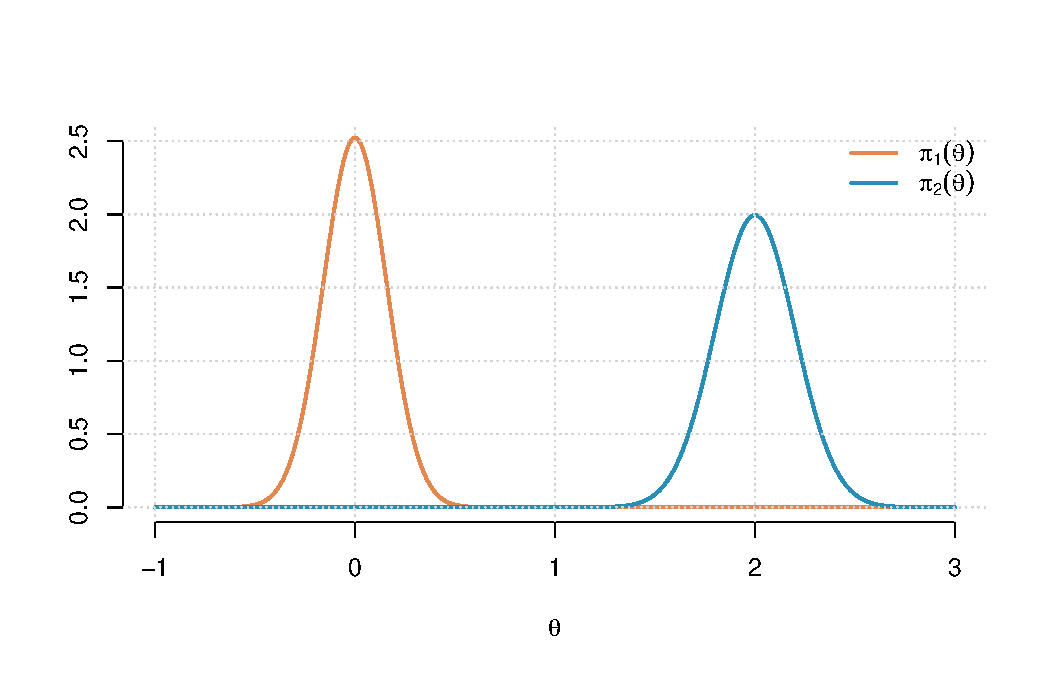
\includegraphics[width = 1\textwidth]{images/plot_priors1.pdf}
\end{figure}
    
\end{frame}



\begin{frame}{A Toy Example}{mildly informative priors}
\[\eta = 0.1 \qquad\qquad\qquad {\color{light}n^*} = 125\]
\begin{figure}
    \centering
    \includegraphics<1>[width = 1\textwidth]{images/plot_PEC11.pdf}
    \includegraphics<2>[width = 1\textwidth]{images/plot_PEC12.pdf}
\end{figure}
    
\end{frame}




\begin{frame}{Another Toy Example}{weakly informative priors}
\[\pi_1(\theta) = \text{N}(0,2/8 ) \qquad\qquad\qquad \pi_2(\theta) = \text{N}(2,2/5 )\]
\begin{figure}
    \centering
    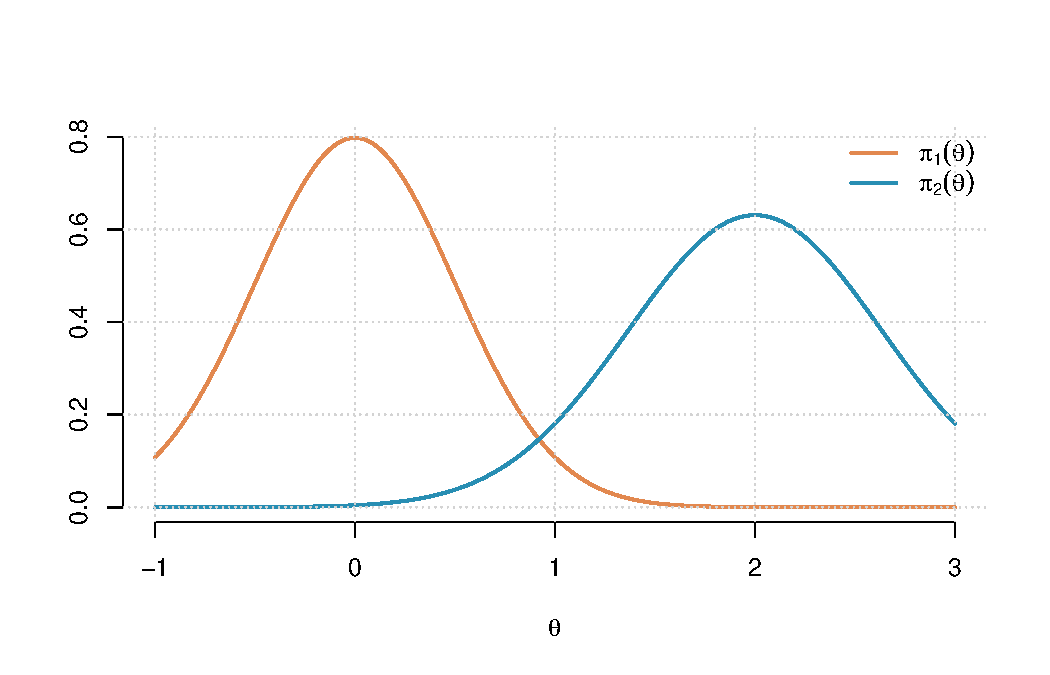
\includegraphics[width = 1\textwidth]{images/plot_priors2.pdf}
\end{figure}
    
\end{frame}



\begin{frame}{Another Toy Example}{weakly informative priors}
\[\eta = 0.1 \qquad\qquad\qquad {\color{light}n^*} = 15\]
\begin{figure}
    \centering
    \includegraphics<1>[width = 1\textwidth]{images/plot_PEC21.pdf}
    \includegraphics<2>[width = 1\textwidth]{images/plot_PEC22.pdf}
\end{figure}
    
\end{frame}


\begin{frame}{How to select $\eta$?}{a small bump in the road}

\begin{exampleblock}

Given a $\beta \in (0,1)$, choose $\eta$ as $$\beta \times \arg\max_n  e_{1,2} (n) $$
\end{exampleblock}

\vspace{0.25cm}

\pause 
It turns out that under some regularity assumptions, $ e_{1,2} (n) $ \textcolor{light}{\bf can be monotone in $n$}. 

\vspace{0.25cm}
\pause 

When this happens 
$$\arg\max_n e_{1,2} (n) =  e_{1,2}(1)$$

$\beta$ represent how much difference we can tolerate with respect to the minimum sample size possible. 

\end{frame}


\begin{frame}{A Toy Example}{Reprise}
    
    \[\eta = 0.1 \qquad\qquad\qquad {\color{light}n^*} = 125\]
\begin{figure}
    \centering
    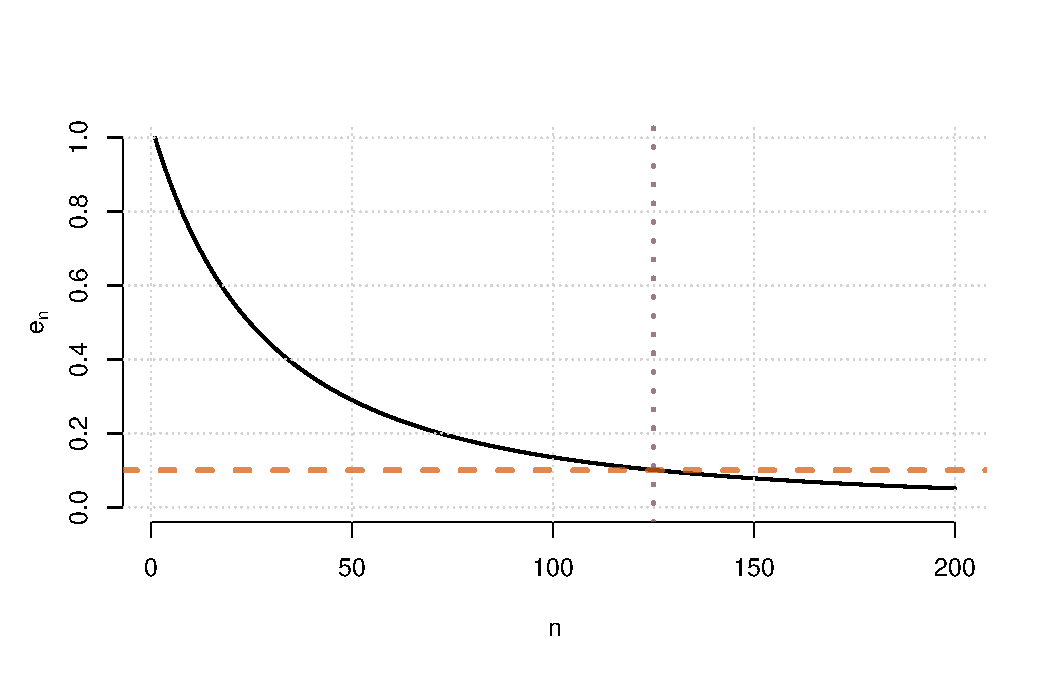
\includegraphics[width = 1\textwidth]{images/plot_PEC12.pdf}
\end{figure}
    
    
\end{frame}


\begin{frame}{A Real Data Example}{from Spiegelhlter et al. (2004)}

$\theta = \log \text{OR}$ of intravenous magnesium sulphate after acute myocardial infarction with respect to placebo.

\vspace{0.25cm}

\pause

A bunch of priors encoding evidence from previous experiments:

\begin{figure}
    \centering
    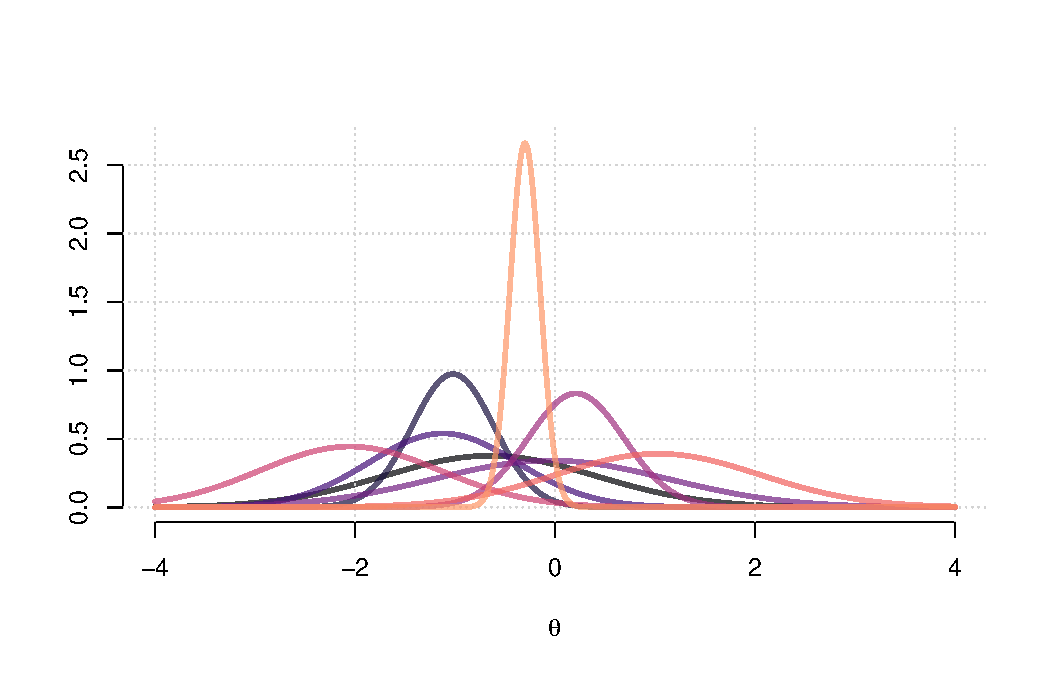
\includegraphics[width = .91\textwidth]{images/plot_mix1.pdf}
\end{figure}
    



\end{frame}

\begin{frame}{An Unfair Comparison}{was this really necessary?}
\begin{itemize}
    \item \textbf{Likelihood} Gaussian with unknown mean $\theta$ and $\sigma^2 = 4$
    \item \textbf{Design Prior} Gaussian with mean $\mu_D = 0.058$ and variance $\sigma^2/n_D$
    \item \textbf{Threshold} $\eta = 0.05$
\end{itemize}

\vspace{0.25cm}

\pause

\begin{table}[]
    \centering
    \begin{tabular}{r|c c c}
    
    \bm{n_D} & \bm{n^*_{\tt WASS}}  &  & \bm{\textcolor<1-2>{white}{$n_{\tt MIXT}^*$}}\\
    & & & \\ 
    4319 & 361 &  & \textcolor<1-2>{white}{$498$}\\
    432 & 371  &  & \textcolor<1-2>{white}{$509$}\\
    43 & 468   &  & \textcolor<1-2>{white}{$190$}
    \end{tabular}
    \label{tab:my_label}
\end{table}

\pause 

\begin{exampleblock}

\begin{center}
Consensus does not typically come ``for free''
\end{center}
\end{exampleblock}

\vspace{0.35cm}

\textcolor[RGB]{220,220,220}{\rule{\linewidth}{0.2pt}}

\tiny{\faBook \;Brutti, P., De Santis, F., \& Gubbiotti, S. (2009). \textit{Mixtures of prior distributions for predictive Bayesian sample size calculations in clinical trials}. Statistics in medicine}
\end{frame}





\begin{frame}{Conjugate Beta-Binomial}{moving beyond gaussianity}

When the posterior distributions are not Gaussian, the Wasserstein distance does not necessarily have an analyitic expression. 

\vspace{0.75cm}

This is the case for the Beta-Binomial conjugate model. 

\vspace{0.75cm}

\pause

Possible solutions are: 
\begin{itemize}
    \item Numerical evaluation of the Wasserstein distance 
    \item Approximation of the Wasserstein distance via Stein's method
\end{itemize}
    
\end{frame}

\begin{frame}{Stein's method}{quickest introduction ever}
    
X, Y random variables (typically X is "what you have", Y is "what you want")
\vspace{0.5cm}

\begin{enumerate}[<+->]
    \item rewrite the distance between $X$ and $Y$ as the \textcolor{light}{\bf expectation} of a functional $h(X)$
    \begin{itemize}
        \item 
    \end{itemize}
    \item \textbf{\color{light} bound} such expectation
\end{enumerate}


\vspace{0.5cm}

\pause 

If we compare $X$ and $Y$ via the $L_1$ Wasserstein distance, we can derive tight bounds for it.

\vspace{0.75cm}


\textcolor[RGB]{220,220,220}{\rule{\linewidth}{0.2pt}}
\tiny{\faBook \; Ley, C., Reinert, G., \& Swan, Y. (2017). Stein’s method for comparison of univariate distributions. \textit{Probability Surveys}.}

\end{frame}


\begin{frame}{Stein's bound for the B-B case}{the second most famous framework in clinical trials}

\textbf{Likelihood:} $\text{Binomial}(\theta, N)$, $T$ events in the sample.


\[ \textcolor<2->{black}{
\pi(\theta) =  \text{Beta}\left(\theta; \alpha, \beta \right)} 
\uncover<2-> {
\qquad \qquad \qquad 
\pi(\theta |y_n) = \text{Beta}\left(\theta; \alpha + t, \beta + n - t \right)}\]

\pause
\pause

\[ d_W(\pi_{1,y}, \pi_{2,y}) \leq \frac{|\alpha_1-\alpha_2|}{\alpha_1 + \beta_1 + n} (1-\mu_{2,P}) + \frac{|\beta_2-\beta_1|}{\alpha_1 + \beta_1 + n}\mu_{2,P}  \]


\pause

\vspace{0.5cm}

If we assume $\pi_D(\theta) = \text{Beta}(\theta; \alpha_D, \beta_D)$ it is possible to bound the \textbf{\color{light} PEC} and \textbf{\color{light}PPC} just by remembering: 

\[\mathbb{E}_{m_D}[T] = \frac{n\alpha_D}{\alpha_D + \beta_D}\]

\end{frame}


\begin{frame}{Yet Another Toy Example}{the more the merrier}
\[\pi_1(\theta) = \text{Beta}(9,  13) \qquad\qquad\qquad \pi_2(\theta) = \text{Beta}(12,4 )\]
\begin{figure}
    \centering
    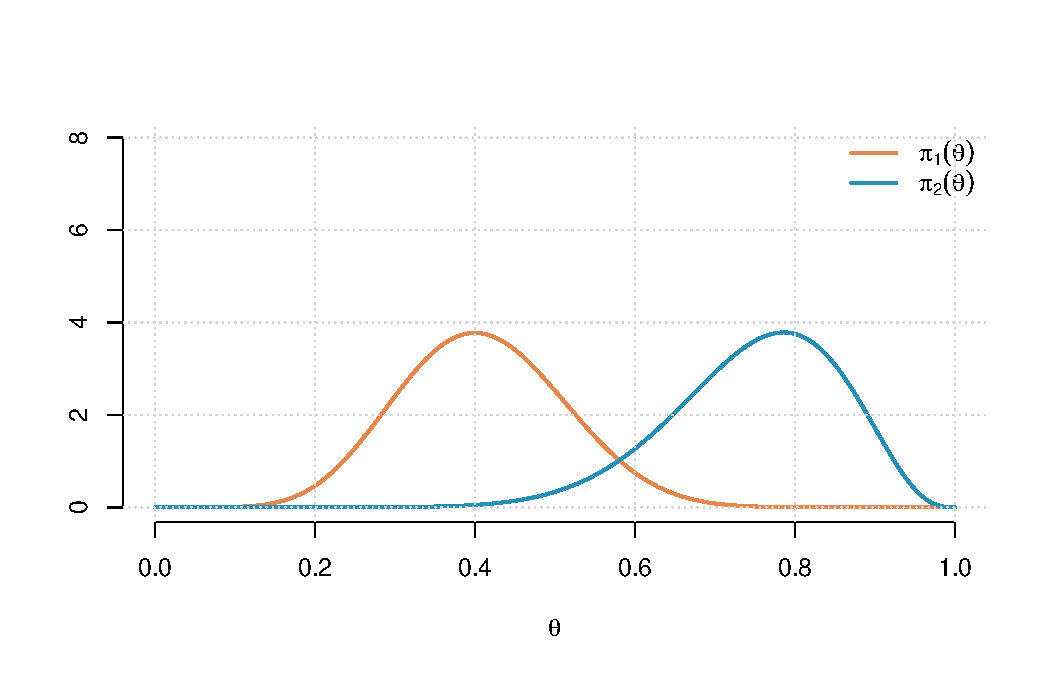
\includegraphics[width = 1\textwidth]{images/plot_priors3.pdf}
\end{figure}
    
\end{frame}


\begin{frame}{Yet Another Toy Example}{the more the merrier}
\[\eta = 0.1 \qquad\qquad\qquad {\color{light}n^*} = 184\]
\begin{figure}
    \centering
    \includegraphics<1>[width = 1\textwidth]{images/plot_PEC32.pdf}
\end{figure}
    
\end{frame}


\begin{frame}

\vspace{1cm}

\Large{\textcolor{light}{\faArchive} \qquad\texttt{R}-package coming soon!}

\begin{tikzpicture}[remember picture,overlay] % Background box
\node [xshift=\paperwidth/2,yshift=\paperheight/2] at (current page.south west)[rectangle,fill,inner sep=0pt,minimum width=\paperwidth,minimum height=\paperheight/3,top color=light!70,bottom color=light!70]{}; % Change the height of the box, its colors and position on the page here
\end{tikzpicture}

\sffamily

\vspace{2cm}

\begin{columns}

\begin{column}{0.45\textwidth}


\includegraphics[width=.7\textwidth]{sapienza-logo-png-6.png}

\vspace{2cm}
{\small 
\textcolor{light}{\faLaptop} \; tulliapadellini.github.io     

\textcolor{light}{\faEnvelope} \; tullia.padellini@uniroma1.it
}


\end{column}

\begin{column}{0.45\textwidth}

\hfill \huge{\color{white} \bf Thanks!}

\vspace{0.25cm}



\vspace{1.25cm}
\vspace{0.3cm}

\small{\hfill } 



\vspace{0.7cm}
\vfill
\hfill 
\end{column}

\end{columns}

\end{frame}

\end{document}
